\usetikzlibrary{shapes}
\usetikzlibrary{arrows}
\usetikzlibrary{calc,positioning}
\begin{figure}
\centering
\scalebox{1}{
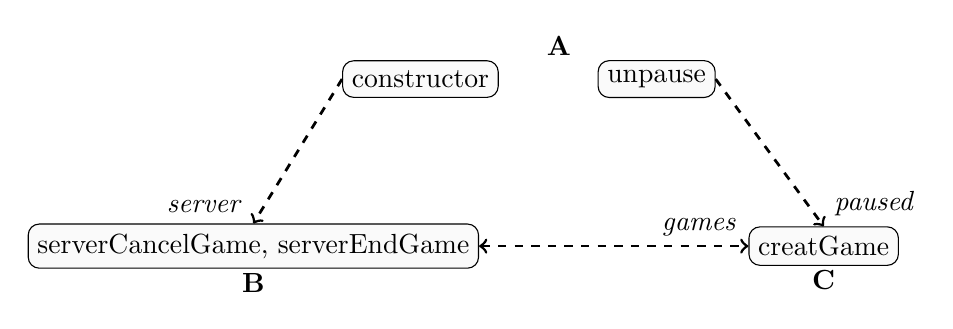
\begin{tikzpicture}[node distance=3cm]
	\tikzstyle{role}=[fill={rgb:black,1;white,50}, draw, rounded corners,
	rectangle split,  
	rectangle split parts=1, 
	rectangle split draw splits=true,  text centered, text width=]
	\node[role] (roleA1) {constructor};
	\node[role] [right of=roleA1] (roleA2) {unpause};
	\node[role] [below right of=roleA2] (roleC) {creatGame};
	\node[role] [below left of=roleA1] (roleB) {serverCancelGame, serverEndGame};

	\draw ([xshift=50pt, yshift=5pt]roleA1.north) node[] {\textbf{A}};
	\draw ([yshift=-5pt]roleB.south) node[] {\textbf{B}};
	\draw ([yshift=-5pt]roleC.south) node[] {\textbf{C}};
	
	\draw [->, dashed, line width=1pt] (roleA1.west) -- (roleB.north) node[above left] {\textit{server}}; 
	\draw [->, dashed, line width=1pt] (roleA2.east) -- (roleC.north)
	node[above right] {\textit{paused}}; 
	; 
	\draw[<->, dashed, line width=1pt] (roleB.east) -- (roleC.west) node[above left] {\textit{games}}; 
	
\end{tikzpicture}
}
\caption{The information flow between roles of Dicether.}
\label{fig: DicetherRoleInformationFlow}
\end{figure}